\ifpdf
    \graphicspath{{Appendix2/Appendix2Figs/PN1G/}{Appendix2/Appendix2Figs/PDF/}{Appendix2/Appendix2Figs/}}
\else
    \graphicspath{{Appendix2/Appendix2Figs/EPS/}{Appendix2/Appendix2Figs/}}
\fi
\setcounter{section}{0}
\chapter{Appendix B}
\markright{Appendix B}
\section{Test Data and Figures}

\begin{figure}[!htbp]
  \begin{center}
    \resizebox{\textwidth}{!}{% This file was created by matlab2tikz v0.4.7 running on MATLAB 8.1.
% Copyright (c) 2008--2014, Nico Schlömer <nico.schloemer@gmail.com>
% All rights reserved.
% Minimal pgfplots version: 1.3
% 
% The latest updates can be retrieved from
%   http://www.mathworks.com/matlabcentral/fileexchange/22022-matlab2tikz
% where you can also make suggestions and rate matlab2tikz.
% 
\begin{tikzpicture}

\begin{axis}[%
width=2.5in,
height=2.5in,
axis on top,
scale only axis,
xmin=0.5,
xmax=200.5,
y dir=reverse,
ymin=0.5,
ymax=200.5,
name=plot2,
title={BPMF $\beta$=5 D=90 RMSE=0.5453}
]
\addplot [forget plot] graphics [xmin=0.5,xmax=200.5,ymin=0.5,ymax=200.5] {test-1.png};
\end{axis}

\begin{axis}[%
width=2.5in,
height=2.5in,
axis on top,
scale only axis,
xmin=0.5,
xmax=200.5,
y dir=reverse,
ymin=0.5,
ymax=200.5,
name=plot1,
at=(plot2.left of south west),
anchor=right of south east,
title={PMF $\lambda$=0.01 D=90 RMSE=0.5046}
]
\addplot [forget plot] graphics [xmin=0.5,xmax=200.5,ymin=0.5,ymax=200.5] {test-2.png};
\end{axis}

\begin{axis}[%
width=2.5in,
height=2.5in,
axis on top,
scale only axis,
xmin=0.5,
xmax=200.5,
y dir=reverse,
ymin=0.5,
ymax=200.5,
name=plot4,
at=(plot1.below south west),
anchor=above north west,
title={PMF $\lambda$=0.1 D=30 RMSE=0.5192}
]
\addplot [forget plot] graphics [xmin=0.5,xmax=200.5,ymin=0.5,ymax=200.5] {test-3.png};
\end{axis}

\begin{axis}[%
width=2.5in,
height=2.5in,
axis on top,
scale only axis,
xmin=0.5,
xmax=200.5,
y dir=reverse,
ymin=0.5,
ymax=200.5,
name=plot5,
at=(plot4.right of south east),
anchor=left of south west,
title={Original Data}
]
\addplot [forget plot] graphics [xmin=0.5,xmax=200.5,ymin=0.5,ymax=200.5] {test-4.png};
\end{axis}

\begin{axis}[%
width=2.5in,
height=2.5in,
axis on top,
scale only axis,
xmin=0.5,
xmax=200.5,
y dir=reverse,
ymin=0.5,
ymax=200.5,
name=plot6,
at=(plot5.right of south east),
anchor=left of south west,
title={Data available to algorithms}
]
\addplot [forget plot] graphics [xmin=0.5,xmax=200.5,ymin=0.5,ymax=200.5] {test-5.png};
\end{axis}

\begin{axis}[%
width=2.5in,
height=2.5in,
axis on top,
scale only axis,
xmin=0.5,
xmax=200.5,
y dir=reverse,
ymin=0.5,
ymax=200.5,
at=(plot6.above north west),
anchor=below south west,
title={KPMF $\sigma$=10 D=90 RMSE=0.6774}
]
\addplot [forget plot] graphics [xmin=0.5,xmax=200.5,ymin=0.5,ymax=200.5] {test-6.png};
\end{axis}
\end{tikzpicture}%}
    \caption{Image Restoration with Matrix Factorisation with 75\% complete data}
    \label{Image Restore}
  \end{center}
\end{figure}

\begin{figure}[!htbp]
  \begin{center}
    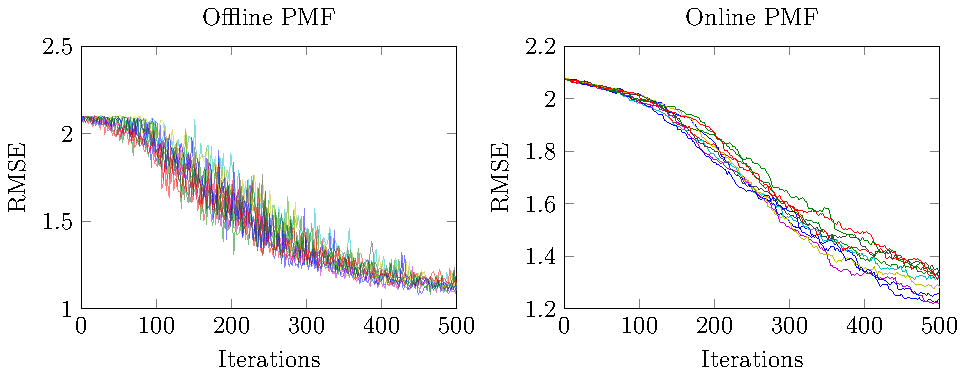
\includegraphics[width=\textwidth]{random_pmf_err}

10 different random sampling simulations on synthetic data.

    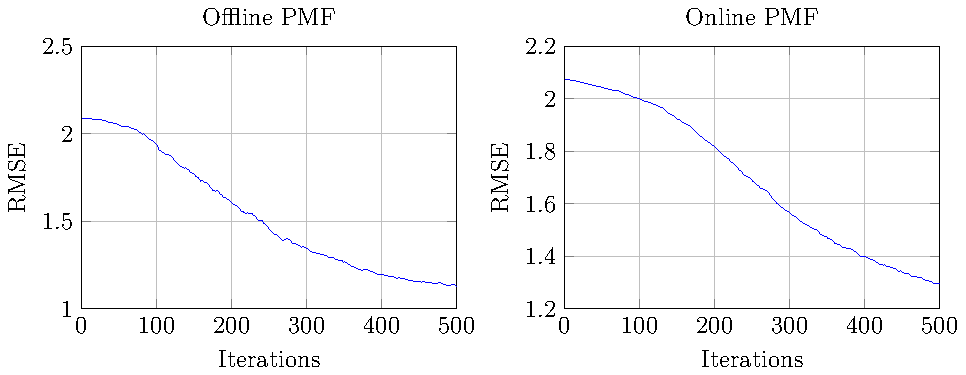
\includegraphics[width=\textwidth]{random_pmf_err_av}
  
Average of 10 simulations.
\end{center}
Original data complete at 1.25\% (with another 1.25\% as validation data)

$\lambda = 0.01$, $D=30$
    \caption{Random Sampling Performance}
    \label{fig:RandomPMF}
\end{figure}


\begin{figure}[!htbp]
  \begin{center}
    \resizebox{\textwidth}{!}{% This file was created by matlab2tikz v0.4.7 running on MATLAB 8.1.
% Copyright (c) 2008--2014, Nico Schlömer <nico.schloemer@gmail.com>
% All rights reserved.
% Minimal pgfplots version: 1.3
% 
% The latest updates can be retrieved from
%   http://www.mathworks.com/matlabcentral/fileexchange/22022-matlab2tikz
% where you can also make suggestions and rate matlab2tikz.
% 
\begin{tikzpicture}

\begin{axis}[%
width=2.20519323671498in,
height=1.97916666666667in,
axis on top,
scale only axis,
xmin=0.5,
xmax=50.5,
y dir=reverse,
ymin=0.5,
ymax=80.5,
name=plot2,
title={Targeted RMSE:1.026}
]
\addplot [forget plot] graphics [xmin=0.5,xmax=50.5,ymin=0.5,ymax=80.5] {eiffel_targeted-1.png};
\end{axis}

\begin{axis}[%
width=2.20519323671498in,
height=1.97916666666667in,
axis on top,
scale only axis,
xmin=0.5,
xmax=50.5,
y dir=reverse,
ymin=0.5,
ymax=80.5,
at=(plot2.left of south west),
anchor=right of south east,
title={Random RMSE:1.150}
]
\addplot [forget plot] graphics [xmin=0.5,xmax=50.5,ymin=0.5,ymax=80.5] {eiffel_targeted-2.png};
\end{axis}

\begin{axis}[%
width=2.20519323671498in,
height=1.97916666666667in,
scale only axis,
xmin=0,
xmax=500,
xlabel={Discovered Samples},
xmajorgrids,
ymin=1,
ymax=2.5,
ylabel={RMSE},
ymajorgrids,
at=(plot2.right of south east),
anchor=left of south west,
title={Target Advantage:1.121},
legend style={draw=black,fill=white,legend cell align=left}
]
\addplot [color=blue,solid]
  table[row sep=crcr]{1	2.31404110645431\\
2	2.31425676410772\\
3	2.31445314839852\\
4	2.31464224670157\\
5	2.3148230859133\\
6	2.31500347878772\\
7	2.31517197314324\\
8	2.31533090214101\\
9	2.31548026212016\\
10	2.31561882833117\\
11	2.31574629352643\\
12	2.31586035565615\\
13	2.31596047556861\\
14	2.31604673729122\\
15	2.31612181590995\\
16	2.31618349045928\\
17	2.31622852518408\\
18	2.31625403286526\\
19	2.31625938910281\\
20	2.31624340397645\\
21	2.31620913357688\\
22	2.31615681412815\\
23	2.31608368123415\\
24	2.31599115706155\\
25	2.31588245005086\\
26	2.31576070749188\\
27	2.3156320303397\\
28	2.31549541257714\\
29	2.31535313799507\\
30	2.31520443325658\\
31	2.31505407474224\\
32	2.31490762190249\\
33	2.31477104322384\\
34	2.31464577823891\\
35	2.31453556266216\\
36	2.31367512137507\\
37	2.31133141183075\\
38	2.30893215992846\\
39	2.30650971262684\\
40	2.30412301276157\\
41	2.30174438542043\\
42	2.29825704023954\\
43	2.29396998338987\\
44	2.28955234333315\\
45	2.28553444213561\\
46	2.28269614348167\\
47	2.27989622368111\\
48	2.27686664953449\\
49	2.27365171102934\\
50	2.27023196965582\\
51	2.26767360984365\\
52	2.26563391361735\\
53	2.26313220664701\\
54	2.26028793925186\\
55	2.25709664736405\\
56	2.25396599323182\\
57	2.25088044068646\\
58	2.24797896815248\\
59	2.24521913427738\\
60	2.24274670183256\\
61	2.23992279056988\\
62	2.23750986731172\\
63	2.23516068852215\\
64	2.23330542066572\\
65	2.23086453116089\\
66	2.2276147279155\\
67	2.22402311282556\\
68	2.21968208736963\\
69	2.21472898482275\\
70	2.21011626628004\\
71	2.20516774286581\\
72	2.20075266788708\\
73	2.1963649015196\\
74	2.19142907996696\\
75	2.18708551114042\\
76	2.18291178800323\\
77	2.17924383977798\\
78	2.17571829649391\\
79	2.1715380888313\\
80	2.16725190729356\\
81	2.16298075377251\\
82	2.15810449879445\\
83	2.15292846205056\\
84	2.14798517609918\\
85	2.14235341644846\\
86	2.13638253886028\\
87	2.12961373481339\\
88	2.1229212739864\\
89	2.11647192798464\\
90	2.11011374985976\\
91	2.10387460599727\\
92	2.09900652328492\\
93	2.09432514790324\\
94	2.08963270718528\\
95	2.08541542179971\\
96	2.08123727813863\\
97	2.07778329008597\\
98	2.07394228885339\\
99	2.06994299047714\\
100	2.06679641801406\\
101	2.06360287140035\\
102	2.06067533630061\\
103	2.05871968567553\\
104	2.05741030392604\\
105	2.05757575632287\\
106	2.05804050046423\\
107	2.05952591243483\\
108	2.06132085158814\\
109	2.06274009832885\\
110	2.0637617846477\\
111	2.06468704623101\\
112	2.06574442631035\\
113	2.06631754050325\\
114	2.06635819082058\\
115	2.06593488729644\\
116	2.06496725444543\\
117	2.06401220274222\\
118	2.0630782332167\\
119	2.06193635207706\\
120	2.06048682458899\\
121	2.05871880217036\\
122	2.0563480204811\\
123	2.05414150344562\\
124	2.05213112336069\\
125	2.04996804171759\\
126	2.04760419035381\\
127	2.04509504656717\\
128	2.04291044538646\\
129	2.04022121803992\\
130	2.0366001720942\\
131	2.03251774271153\\
132	2.02822169638034\\
133	2.02391300233605\\
134	2.02002760422263\\
135	2.01599156130752\\
136	2.01200496345005\\
137	2.00821986163712\\
138	2.00482293919736\\
139	2.00174458210825\\
140	1.99971890284615\\
141	1.99789641480728\\
142	1.9957113768081\\
143	1.99353458222666\\
144	1.99059396165287\\
145	1.98675682851332\\
146	1.98317966584436\\
147	1.9801327821626\\
148	1.97764453794438\\
149	1.9753179673464\\
150	1.97258209449641\\
151	1.9699980130529\\
152	1.96605677583408\\
153	1.96295453677439\\
154	1.96098705423561\\
155	1.95881944915206\\
156	1.95552175575229\\
157	1.9522892400729\\
158	1.947695534894\\
159	1.94338425183434\\
160	1.93944218286694\\
161	1.93696704180037\\
162	1.93398755698765\\
163	1.93069293982857\\
164	1.92656934096279\\
165	1.92218081730403\\
166	1.91706703784556\\
167	1.91277626882804\\
168	1.90787895696652\\
169	1.90220432406231\\
170	1.89624521080799\\
171	1.89238799984753\\
172	1.88754110395697\\
173	1.88328154031879\\
174	1.88015771048206\\
175	1.87741123515482\\
176	1.87496408674419\\
177	1.87348107542113\\
178	1.87191880507184\\
179	1.87017675864246\\
180	1.86636775725631\\
181	1.86310983159721\\
182	1.85947747265745\\
183	1.8555827401434\\
184	1.85105978090019\\
185	1.84631313994686\\
186	1.84005709784503\\
187	1.8332499095589\\
188	1.82598753773178\\
189	1.81881957264238\\
190	1.81224096037214\\
191	1.80618699488285\\
192	1.80033034533977\\
193	1.79532785916755\\
194	1.79060556210099\\
195	1.78732780682547\\
196	1.78556853519003\\
197	1.78405362022411\\
198	1.78297399133508\\
199	1.78148452879606\\
200	1.77996510610784\\
201	1.77829005674299\\
202	1.7764929442072\\
203	1.77429300771002\\
204	1.7714152201878\\
205	1.76868676240815\\
206	1.7668056822737\\
207	1.76522125238592\\
208	1.76455179919605\\
209	1.76420858677775\\
210	1.76455393958375\\
211	1.76523335023632\\
212	1.76538461489872\\
213	1.76597837651021\\
214	1.76620173405808\\
215	1.76546532651268\\
216	1.76396082815346\\
217	1.76214145061607\\
218	1.76026773391705\\
219	1.75743840369648\\
220	1.75287278411311\\
221	1.74860158866225\\
222	1.7422724987361\\
223	1.73462323404525\\
224	1.72694205025914\\
225	1.71843061991188\\
226	1.70951811417603\\
227	1.69986192414951\\
228	1.68962918229449\\
229	1.68057605031386\\
230	1.67150501766814\\
231	1.66400684376912\\
232	1.65655022903279\\
233	1.64960011995681\\
234	1.64397254066184\\
235	1.63795198071727\\
236	1.63219735421561\\
237	1.62577826333049\\
238	1.61870022642254\\
239	1.61104620172168\\
240	1.60377773687994\\
241	1.59726499495644\\
242	1.59081340798708\\
243	1.58294438009457\\
244	1.5748601183041\\
245	1.56700968406842\\
246	1.55898839455494\\
247	1.55013000234112\\
248	1.54206085435789\\
249	1.53472855290209\\
250	1.52785969041305\\
251	1.52064555367461\\
252	1.51460723671974\\
253	1.50922398293897\\
254	1.50395232977853\\
255	1.50077181553249\\
256	1.49974426459448\\
257	1.49934957451923\\
258	1.4986769691068\\
259	1.49678699654613\\
260	1.49533445058535\\
261	1.4940934887377\\
262	1.49336170207339\\
263	1.49236686793284\\
264	1.49130382239467\\
265	1.4893922274161\\
266	1.48793352060723\\
267	1.48495389929656\\
268	1.48314301738427\\
269	1.48014285084888\\
270	1.47775221171514\\
271	1.47476598856971\\
272	1.47187322300268\\
273	1.46856816159847\\
274	1.46529818280839\\
275	1.46111021993423\\
276	1.4576935276672\\
277	1.45436240615844\\
278	1.45096899407841\\
279	1.44459474276816\\
280	1.43784659108841\\
281	1.43092243207188\\
282	1.42426220456286\\
283	1.41814043602794\\
284	1.41218729563923\\
285	1.40651477340576\\
286	1.40045352950293\\
287	1.39548242948141\\
288	1.39286901396478\\
289	1.3910515719995\\
290	1.38924755035503\\
291	1.38737689176505\\
292	1.38590022022086\\
293	1.38458249045794\\
294	1.38328453455804\\
295	1.38254836201366\\
296	1.38108533644439\\
297	1.37954055278099\\
298	1.3776923532805\\
299	1.37575120062471\\
300	1.37377388163956\\
301	1.37093306748052\\
302	1.36766933434279\\
303	1.36329401718814\\
304	1.35849014149051\\
305	1.35478622889932\\
306	1.35049390680744\\
307	1.34586286295709\\
308	1.34163124354616\\
309	1.33766768026547\\
310	1.33386724219489\\
311	1.32943490937536\\
312	1.32614031863094\\
313	1.32249266607618\\
314	1.31798137336285\\
315	1.31377392077356\\
316	1.30955420575781\\
317	1.30506928628429\\
318	1.3001843878094\\
319	1.29474511316326\\
320	1.28934435535143\\
321	1.28198062559397\\
322	1.27462383842209\\
323	1.26716352049109\\
324	1.25887633674218\\
325	1.25112835303693\\
326	1.24336672130161\\
327	1.23454177718307\\
328	1.22622188281774\\
329	1.21778876855187\\
330	1.21106760667605\\
331	1.2054302957322\\
332	1.2002172877545\\
333	1.19623728555625\\
334	1.1924473615307\\
335	1.18859067361414\\
336	1.18607494982103\\
337	1.18430580723422\\
338	1.18366502803976\\
339	1.18314272926967\\
340	1.18173438363381\\
341	1.1819971420057\\
342	1.18233657371344\\
343	1.18186810205928\\
344	1.18169818328992\\
345	1.17908462155883\\
346	1.17597464040899\\
347	1.17300140750746\\
348	1.16937264513645\\
349	1.16622900615379\\
350	1.16271980237193\\
351	1.15831341790407\\
352	1.15453229329104\\
353	1.15118918566305\\
354	1.1500019860983\\
355	1.14870343679925\\
356	1.14678494281984\\
357	1.14608200911847\\
358	1.14524409793541\\
359	1.14302371321857\\
360	1.14157043595355\\
361	1.14015680719264\\
362	1.13808846556812\\
363	1.13653692457014\\
364	1.13544875888625\\
365	1.13499696672541\\
366	1.13446572014099\\
367	1.13405179565849\\
368	1.13412112512648\\
369	1.13452300223401\\
370	1.13480353107401\\
371	1.1338669722912\\
372	1.13294576232921\\
373	1.132210338563\\
374	1.13071617048058\\
375	1.12914031490681\\
376	1.128124706498\\
377	1.12744817632259\\
378	1.12556482665768\\
379	1.12443979316368\\
380	1.12478371786562\\
381	1.12488314142209\\
382	1.12471185282376\\
383	1.12510422313935\\
384	1.12535745156609\\
385	1.12506060368295\\
386	1.12434607261844\\
387	1.12478231671223\\
388	1.12441408052388\\
389	1.12374740746535\\
390	1.12307245067258\\
391	1.12224135194087\\
392	1.1215611240691\\
393	1.1210098422898\\
394	1.12034029137756\\
395	1.11933093895885\\
396	1.11756155263503\\
397	1.11584301135065\\
398	1.11442383961708\\
399	1.11276340231533\\
400	1.11089757263032\\
401	1.10927453118418\\
402	1.10791579506042\\
403	1.10744268242344\\
404	1.10732375320097\\
405	1.1074633022322\\
406	1.10806357081508\\
407	1.10793646890823\\
408	1.10794014435402\\
409	1.10839819512728\\
410	1.10730938175033\\
411	1.10617439324513\\
412	1.10453466388317\\
413	1.10304768922282\\
414	1.10301761356726\\
415	1.10279732761721\\
416	1.10375828039174\\
417	1.10436974558807\\
418	1.10426536456825\\
419	1.10464643864108\\
420	1.1044447879411\\
421	1.10365653993683\\
422	1.10256528887274\\
423	1.09943096337995\\
424	1.09615128131274\\
425	1.09167467091655\\
426	1.08679093852122\\
427	1.08156201467031\\
428	1.07693291616992\\
429	1.07325532038483\\
430	1.0706171877207\\
431	1.06827479097178\\
432	1.06705310232508\\
433	1.0657078321307\\
434	1.06575731746021\\
435	1.06684691277451\\
436	1.06888355298626\\
437	1.07103008848007\\
438	1.07254064176797\\
439	1.07328740480429\\
440	1.07307719095926\\
441	1.07213068209425\\
442	1.07198310934042\\
443	1.07127118163626\\
444	1.06952555473331\\
445	1.06792544667732\\
446	1.0661196179934\\
447	1.06417255961584\\
448	1.06270293503517\\
449	1.06209465557552\\
450	1.06209292254494\\
451	1.06160732920945\\
452	1.06112383559056\\
453	1.06111994158496\\
454	1.06113358993323\\
455	1.06100267653073\\
456	1.06139992254746\\
457	1.06113685194682\\
458	1.06089072855103\\
459	1.06065937068311\\
460	1.06058574796627\\
461	1.06024130901433\\
462	1.06004417084353\\
463	1.05980345998416\\
464	1.05931545814962\\
465	1.05805228352948\\
466	1.05652533583289\\
467	1.05469460630483\\
468	1.05255148442967\\
469	1.04970406114713\\
470	1.04712866146986\\
471	1.04453784588575\\
472	1.04153123897601\\
473	1.039413252842\\
474	1.03765015459116\\
475	1.03641738638663\\
476	1.03532465856552\\
477	1.03374122849738\\
478	1.03258515498343\\
479	1.03134414645722\\
480	1.03024344178858\\
481	1.02961201270084\\
482	1.02847522014646\\
483	1.02696751681409\\
484	1.02520036828126\\
485	1.02337445197715\\
486	1.02168885737384\\
487	1.01919851361261\\
488	1.01650833460998\\
489	1.01382105523529\\
490	1.01112603215788\\
491	1.00840923638358\\
492	1.00590052369843\\
493	1.00589367775222\\
494	1.00761346036835\\
495	1.00919069115692\\
496	1.01159515941495\\
497	1.01459282615493\\
498	1.01999106895151\\
499	1.02786397477042\\
500	1.02605019636602\\
};
\addlegendentry{Random Sampling};

\addplot [color=black!50!green,solid]
  table[row sep=crcr]{1	2.31355651732015\\
2	2.31356566020658\\
3	2.31323047111064\\
4	2.31247525805625\\
5	2.31193696428279\\
6	2.31145193854417\\
7	2.31093760321731\\
8	2.31043973508214\\
9	2.30986109424655\\
10	2.3093435655076\\
11	2.30898671085035\\
12	2.30864489318465\\
13	2.30820843383207\\
14	2.30775296516415\\
15	2.3073548669485\\
16	2.3068288178598\\
17	2.30619055608816\\
18	2.3057069522827\\
19	2.30520927923926\\
20	2.30475000571301\\
21	2.30413569269437\\
22	2.30352414106385\\
23	2.30301512054566\\
24	2.3024955382434\\
25	2.30193859105076\\
26	2.30153708217051\\
27	2.3010051379223\\
28	2.30051534877654\\
29	2.29994291447892\\
30	2.29945023083487\\
31	2.29907116399319\\
32	2.29863697599032\\
33	2.29788191061376\\
34	2.29726981760918\\
35	2.29651062249013\\
36	2.29585655690555\\
37	2.29517344939967\\
38	2.29456680352742\\
39	2.29402472387361\\
40	2.29351516122654\\
41	2.29302829618564\\
42	2.29288682775964\\
43	2.29271841968344\\
44	2.29235791588622\\
45	2.29201660391197\\
46	2.2915751014021\\
47	2.29103424305738\\
48	2.29055564978351\\
49	2.29003343570519\\
50	2.28943130927127\\
51	2.28886570753181\\
52	2.28833922852935\\
53	2.28818564129896\\
54	2.28799540746367\\
55	2.28789202646634\\
56	2.28771875306846\\
57	2.28750145398787\\
58	2.28728428827398\\
59	2.28710510092621\\
60	2.28670656189732\\
61	2.28634603564762\\
62	2.28588314710729\\
63	2.28541111526559\\
64	2.28494262057855\\
65	2.28453364231402\\
66	2.28413089674552\\
67	2.28359477312381\\
68	2.28302093814265\\
69	2.28268708600367\\
70	2.28223511042373\\
71	2.28176184232033\\
72	2.28126717242594\\
73	2.28079297446668\\
74	2.2803656355735\\
75	2.27969874316544\\
76	2.27903953062867\\
77	2.27846202017233\\
78	2.27756814411681\\
79	2.27681290586573\\
80	2.27597403032839\\
81	2.27513707695037\\
82	2.27402024188753\\
83	2.27294902076212\\
84	2.27199835395819\\
85	2.2710276898839\\
86	2.2697347194763\\
87	2.26879429251342\\
88	2.26784079969352\\
89	2.26677967604171\\
90	2.26557021962211\\
91	2.26466243103099\\
92	2.26381607500521\\
93	2.26311471463644\\
94	2.26244964810105\\
95	2.26186807087349\\
96	2.26076155132473\\
97	2.25963258314019\\
98	2.25875329679297\\
99	2.25791141761088\\
100	2.25686573858731\\
101	2.25572592405795\\
102	2.25454928031301\\
103	2.25336322475232\\
104	2.25250255897708\\
105	2.25187232412626\\
106	2.25134479889169\\
107	2.25071510560578\\
108	2.25017918279445\\
109	2.2496880591161\\
110	2.24925324488465\\
111	2.24873767854012\\
112	2.2480038241248\\
113	2.24726301382025\\
114	2.2463969005488\\
115	2.24525240300209\\
116	2.24364835947216\\
117	2.24207123746162\\
118	2.24055931690706\\
119	2.2389567149643\\
120	2.23732229795761\\
121	2.23573699257113\\
122	2.23388171450245\\
123	2.23230185160125\\
124	2.23056109236963\\
125	2.22920217097624\\
126	2.22769863239408\\
127	2.22622243126376\\
128	2.22488642875253\\
129	2.22344695353128\\
130	2.22241580881377\\
131	2.22132801809208\\
132	2.21983992700348\\
133	2.2188245202822\\
134	2.21786568663174\\
135	2.21717745623723\\
136	2.2162851450052\\
137	2.21530871655536\\
138	2.21421916340668\\
139	2.21295558426731\\
140	2.21160435511528\\
141	2.21067295864196\\
142	2.20881540464901\\
143	2.20666734262386\\
144	2.20441060304785\\
145	2.20198414893878\\
146	2.19952582066733\\
147	2.19721614269807\\
148	2.19463938148753\\
149	2.19215652308599\\
150	2.18965317861941\\
151	2.18756822103205\\
152	2.18583830802001\\
153	2.18383660214736\\
154	2.18197198507573\\
155	2.18031696791109\\
156	2.17888854851298\\
157	2.17756213707072\\
158	2.17584279038011\\
159	2.17392945355654\\
160	2.17194265066163\\
161	2.16922434846855\\
162	2.16646160304178\\
163	2.1637116361189\\
164	2.16082364107209\\
165	2.15734057141862\\
166	2.15415698703494\\
167	2.1514066367975\\
168	2.14890651673209\\
169	2.14615350277454\\
170	2.14413273742008\\
171	2.14226017846\\
172	2.13968757996299\\
173	2.13661498013055\\
174	2.13333588295244\\
175	2.1300507050753\\
176	2.12630887857031\\
177	2.12224582471576\\
178	2.11867192574391\\
179	2.11507407032549\\
180	2.11098507086203\\
181	2.10770840563658\\
182	2.104889290405\\
183	2.10235072708847\\
184	2.09951807674364\\
185	2.0972354818042\\
186	2.09493842382219\\
187	2.09235206888047\\
188	2.08900492840267\\
189	2.08606462750574\\
190	2.08312144461488\\
191	2.07977788123497\\
192	2.07594546043688\\
193	2.07211457762552\\
194	2.0681843622986\\
195	2.06414321669297\\
196	2.0604906162847\\
197	2.05753233894327\\
198	2.05423201899248\\
199	2.05069876932702\\
200	2.0473679821959\\
201	2.04481918340028\\
202	2.04213791189998\\
203	2.0390743216435\\
204	2.03626366356825\\
205	2.03344259229105\\
206	2.0296496053707\\
207	2.02654219782157\\
208	2.02333550605557\\
209	2.01963165431823\\
210	2.01598638265753\\
211	2.01245431170046\\
212	2.0095302379501\\
213	2.00627564993958\\
214	2.00267460524632\\
215	1.99927350947372\\
216	1.99545176179751\\
217	1.99212371143856\\
218	1.98913316041108\\
219	1.98537883499722\\
220	1.98155635848432\\
221	1.97741610291749\\
222	1.97382064045637\\
223	1.97017401900578\\
224	1.96711881540769\\
225	1.96430821015927\\
226	1.96141564832038\\
227	1.958557223124\\
228	1.95586161344697\\
229	1.95321428321351\\
230	1.95005995767043\\
231	1.94599291440712\\
232	1.94224746827753\\
233	1.93889185079\\
234	1.9349160046348\\
235	1.93013694909405\\
236	1.92471823088953\\
237	1.91993477586086\\
238	1.91466202965007\\
239	1.90985163871627\\
240	1.90455524692571\\
241	1.89900895505723\\
242	1.89326806440131\\
243	1.88814590029984\\
244	1.88326580482791\\
245	1.87883905898706\\
246	1.87425890519452\\
247	1.87025848495357\\
248	1.86614586161227\\
249	1.86331840911406\\
250	1.86071537435874\\
251	1.85796650288101\\
252	1.8547408156344\\
253	1.85080737366106\\
254	1.84665078127658\\
255	1.84256870039945\\
256	1.83861585051675\\
257	1.83465159601838\\
258	1.82973671167983\\
259	1.82400045341437\\
260	1.81822594015466\\
261	1.81227032416754\\
262	1.80743203667508\\
263	1.80275653585674\\
264	1.79683008994035\\
265	1.79063059871071\\
266	1.78427029327884\\
267	1.77833648132276\\
268	1.77361240352778\\
269	1.76842008591514\\
270	1.76389218607563\\
271	1.75886923726544\\
272	1.75405254603892\\
273	1.75066941134979\\
274	1.7477370775049\\
275	1.74453956434007\\
276	1.74127279251289\\
277	1.73738817239367\\
278	1.73415377285533\\
279	1.73099936742665\\
280	1.72738630448789\\
281	1.72360531961805\\
282	1.71896026865338\\
283	1.71411201511617\\
284	1.70979863797483\\
285	1.70519048249347\\
286	1.70087936184304\\
287	1.69590395804856\\
288	1.6911186405967\\
289	1.68697888833162\\
290	1.68214326790307\\
291	1.67743869335299\\
292	1.67083854877209\\
293	1.66462757707148\\
294	1.65866560560533\\
295	1.65227835438196\\
296	1.64715820248178\\
297	1.64152075278102\\
298	1.63621000524499\\
299	1.62965407947917\\
300	1.62371612644748\\
301	1.61951417326594\\
302	1.61332497433663\\
303	1.60883886710821\\
304	1.60478796805914\\
305	1.59966460807922\\
306	1.5940661309777\\
307	1.58860722800978\\
308	1.58481146956848\\
309	1.58095711321011\\
310	1.57677553295084\\
311	1.57441617524935\\
312	1.57056676613693\\
313	1.56688659176\\
314	1.56392603430254\\
315	1.561750734419\\
316	1.55820990489985\\
317	1.55576847191101\\
318	1.55360732752056\\
319	1.55154203165938\\
320	1.54884192548582\\
321	1.54646641493389\\
322	1.54366942364416\\
323	1.54046459151378\\
324	1.53697110487591\\
325	1.5354765525073\\
326	1.53361153397819\\
327	1.5314066375921\\
328	1.52963474571191\\
329	1.52648326253657\\
330	1.52298013008416\\
331	1.51795679651879\\
332	1.51310225213702\\
333	1.50871799102033\\
334	1.50376595715692\\
335	1.49873932647599\\
336	1.49280938967234\\
337	1.4863361877881\\
338	1.48166767130697\\
339	1.47736447537105\\
340	1.47387018589748\\
341	1.47054689114904\\
342	1.46610408819733\\
343	1.46081470600565\\
344	1.45486404158116\\
345	1.45026723130047\\
346	1.44610228283337\\
347	1.44152533000746\\
348	1.43619611716834\\
349	1.4311557371892\\
350	1.42562613008549\\
351	1.4207122329411\\
352	1.41650240542642\\
353	1.41305398323408\\
354	1.40915033939929\\
355	1.40540508037387\\
356	1.40150969069792\\
357	1.39800144746147\\
358	1.39475162841027\\
359	1.3919500355791\\
360	1.38914433808517\\
361	1.386423698983\\
362	1.38284605066004\\
363	1.37941175521707\\
364	1.37575801931725\\
365	1.37320810514657\\
366	1.37112538095449\\
367	1.36783687539288\\
368	1.36441412118992\\
369	1.36113338263728\\
370	1.3579560438647\\
371	1.35468091401008\\
372	1.35020457016068\\
373	1.34611497351895\\
374	1.34111855903329\\
375	1.33516199651132\\
376	1.33145801863336\\
377	1.32818208120271\\
378	1.32567420348368\\
379	1.32217228766702\\
380	1.31964647284392\\
381	1.31816388305518\\
382	1.31583119173864\\
383	1.31351763448467\\
384	1.31202299607488\\
385	1.31056639349238\\
386	1.30826900045043\\
387	1.30523035684101\\
388	1.30288138884817\\
389	1.30093762171791\\
390	1.29919037542968\\
391	1.29811075128451\\
392	1.2974738594748\\
393	1.29711022871794\\
394	1.2964452310665\\
395	1.29533623856166\\
396	1.2946520691074\\
397	1.29424866093843\\
398	1.29351565681501\\
399	1.29217918793326\\
400	1.29083999199595\\
401	1.28925463990045\\
402	1.28794199039559\\
403	1.28593205195636\\
404	1.28466638407692\\
405	1.28312433490653\\
406	1.28103104161751\\
407	1.27903128629618\\
408	1.27802180788597\\
409	1.27770980550536\\
410	1.27784576679104\\
411	1.27741453962001\\
412	1.27742121002841\\
413	1.27780035373636\\
414	1.27794515392025\\
415	1.27803689352109\\
416	1.27819249138332\\
417	1.27737542603794\\
418	1.2759607006949\\
419	1.2738828867809\\
420	1.27140033592091\\
421	1.26685396905252\\
422	1.26228056154393\\
423	1.2576233407123\\
424	1.25288458626841\\
425	1.24709661094785\\
426	1.24202231376621\\
427	1.2367316677216\\
428	1.23367805614844\\
429	1.23143821712816\\
430	1.23132470414198\\
431	1.23115382844202\\
432	1.23100088575675\\
433	1.2314537007536\\
434	1.23229911512576\\
435	1.23293909744274\\
436	1.23367727907891\\
437	1.23307984357647\\
438	1.23206684418599\\
439	1.2309110534019\\
440	1.22987252513006\\
441	1.22913957989914\\
442	1.22887892265067\\
443	1.22829587705842\\
444	1.22757450227168\\
445	1.22597517797487\\
446	1.22400538888464\\
447	1.22388583392221\\
448	1.22373458451004\\
449	1.2233521087221\\
450	1.22263785526085\\
451	1.22131852412864\\
452	1.22062026386659\\
453	1.22021292428176\\
454	1.22033195199516\\
455	1.22052368021259\\
456	1.21910421187171\\
457	1.21675382408037\\
458	1.21413943195238\\
459	1.21161529390472\\
460	1.20913328073211\\
461	1.20583117941093\\
462	1.20261026283376\\
463	1.19988553048394\\
464	1.19728789330464\\
465	1.19408323906272\\
466	1.19312738840717\\
467	1.19190374852315\\
468	1.19167086161593\\
469	1.19119287651117\\
470	1.19092384476178\\
471	1.19046602519544\\
472	1.18993201988666\\
473	1.18934112757251\\
474	1.18934462673543\\
475	1.18894310518462\\
476	1.1886832344409\\
477	1.18760710819821\\
478	1.18659014254121\\
479	1.18648505220062\\
480	1.18636317524915\\
481	1.18638130170429\\
482	1.18633115092021\\
483	1.18564678128192\\
484	1.18381768014321\\
485	1.18231248589041\\
486	1.18085508989434\\
487	1.17852263282527\\
488	1.17582717816612\\
489	1.1722988935254\\
490	1.17012608816856\\
491	1.16824489926652\\
492	1.16577577368752\\
493	1.16353777731863\\
494	1.16130843133576\\
495	1.15904659832518\\
496	1.15760989371068\\
497	1.15788520543675\\
498	1.15415533619797\\
499	1.15273699895913\\
500	1.1501807272355\\
};
\addlegendentry{Targeted};

\end{axis}
\end{tikzpicture}%}
\end{center}
Original data complete at 1.25\% (with another 1.25\% as validation data)

Data is downsampled and rounded Eiffel tower image to fit $[1,5]$.

Online PMF, $\lambda = 0.01$, $D=30$
    \caption{Minimum Knowledge Search on Eiffel Tower}
    \label{fig:eiffel_active_mks}
\end{figure}

\begin{figure}[!htbp]
  \begin{center}
  \resizebox{\textwidth}{!}{% This file was created by matlab2tikz v0.4.7 running on MATLAB 8.1.
% Copyright (c) 2008--2014, Nico Schlömer <nico.schloemer@gmail.com>
% All rights reserved.
% Minimal pgfplots version: 1.3
% 
% The latest updates can be retrieved from
%   http://www.mathworks.com/matlabcentral/fileexchange/22022-matlab2tikz
% where you can also make suggestions and rate matlab2tikz.
% 
\begin{tikzpicture}

\begin{axis}[%
width=2.22901570048309in,
height=2.67421875in,
scale only axis,
xmin=0,
xmax=500,
xlabel={Discovered Samples},
xmajorgrids,
ymin=1,
ymax=2.4,
ylabel={RMSE},
ymajorgrids,
name=plot2,
title={Target Advantage:1.036}
]
\addplot [color=blue,solid,forget plot]
  table[row sep=crcr]{1	2.08955683240127\\
4	2.08120851852688\\
7	2.07534150943872\\
10	2.07113303496436\\
13	2.06449693474286\\
16	2.05704264681726\\
19	2.05270905397449\\
22	2.04703296014939\\
25	2.04208407964867\\
28	2.04378475917784\\
31	2.04058668635071\\
34	2.03556993833398\\
37	2.03064629409764\\
40	2.02436925212641\\
43	2.01630214197685\\
46	2.00858306459747\\
49	2.00474788950457\\
52	1.99800714102804\\
55	1.99003168036556\\
58	1.98764933705001\\
61	1.98809106918327\\
64	1.98630261502406\\
67	1.99195388990038\\
70	1.98620506412944\\
73	1.98445532070391\\
76	1.98382450546172\\
79	1.98455966024057\\
82	1.97646683456422\\
85	1.96064124215243\\
88	1.95283686987202\\
91	1.93738612400345\\
94	1.93214600524994\\
97	1.91391960242186\\
100	1.91008773200848\\
103	1.89804432538063\\
106	1.88349742225093\\
109	1.86923963085806\\
112	1.85975494582399\\
115	1.84732426623339\\
118	1.8398495885267\\
121	1.832029971429\\
124	1.83430118916913\\
127	1.80795489907222\\
130	1.77619551220851\\
133	1.75970980909346\\
136	1.7363092025138\\
139	1.7308471324561\\
142	1.7189590414173\\
145	1.71191578824767\\
148	1.70437376954023\\
151	1.70916406262316\\
154	1.68804972090553\\
157	1.67252104282444\\
160	1.6456634847308\\
163	1.6189741819892\\
166	1.60464948168617\\
169	1.60621676416582\\
172	1.57284008241142\\
175	1.55963179728716\\
178	1.56046771701689\\
181	1.54846115155033\\
184	1.53460295704343\\
187	1.50195343564028\\
190	1.51350246604894\\
193	1.50136850325632\\
196	1.500017435562\\
199	1.48872959731716\\
202	1.45955281676692\\
205	1.45183610033175\\
208	1.44470401288984\\
211	1.43038999419091\\
214	1.41621633424817\\
217	1.40895193528978\\
220	1.40490722731198\\
223	1.396597683391\\
226	1.37752238107544\\
229	1.37177035643585\\
232	1.3698549459506\\
235	1.36553827006921\\
238	1.35426931375028\\
241	1.34750221013096\\
244	1.34244396515889\\
247	1.34136835659876\\
250	1.32563093220512\\
253	1.32325186841771\\
256	1.31697368837166\\
259	1.31529664088897\\
262	1.30886539752246\\
265	1.30108529262825\\
268	1.29502695609685\\
271	1.29228516232994\\
274	1.28792343170974\\
277	1.27880846069708\\
280	1.26935057885263\\
283	1.26864585571813\\
286	1.26427846155713\\
289	1.2591742299134\\
292	1.26431376521135\\
295	1.26994369095501\\
298	1.27092981547445\\
301	1.26880710014083\\
304	1.26349607498073\\
307	1.25935107064976\\
310	1.2548235719608\\
313	1.25282164688069\\
316	1.24925235677718\\
319	1.24874124430829\\
322	1.25197381221379\\
325	1.25266164126656\\
328	1.24966641544741\\
331	1.2443374114334\\
334	1.24173225322926\\
337	1.23843352871422\\
340	1.23818825005499\\
343	1.23902379365268\\
346	1.23499772792284\\
349	1.23310897961122\\
352	1.23218725326399\\
355	1.23832991175924\\
358	1.238352173016\\
361	1.23102789884616\\
364	1.23171407062859\\
367	1.23140279669778\\
370	1.23099437531552\\
373	1.2311049103155\\
376	1.22607044586302\\
379	1.21978483012963\\
382	1.22116626892908\\
385	1.21695925522813\\
388	1.21708073601571\\
391	1.21110506887662\\
394	1.20724445965935\\
397	1.20642265008572\\
400	1.20622462881926\\
403	1.20412882474165\\
406	1.20083061242515\\
409	1.19837280792117\\
412	1.20172505403672\\
415	1.20319101683298\\
418	1.20191803799231\\
421	1.19830110356644\\
424	1.20109288641826\\
427	1.20291675388244\\
430	1.20261455828073\\
433	1.19846430481434\\
436	1.19890943711771\\
439	1.19618381857365\\
442	1.1904762367084\\
445	1.18813768343454\\
448	1.18471312579485\\
451	1.1864199656993\\
454	1.18810129570592\\
457	1.18920911889499\\
460	1.18916307499863\\
463	1.18851670119718\\
466	1.18460260788554\\
469	1.17787772718249\\
472	1.16776406720888\\
475	1.16028534380028\\
478	1.15724755862622\\
481	1.15250980635763\\
484	1.14852187450615\\
487	1.14589696645781\\
490	1.14618821808225\\
493	1.14132401541564\\
496	1.13114833734571\\
499	1.13285082354089\\
500	1.08992714273505\\
};
\addplot [color=black!50!green,solid,forget plot]
  table[row sep=crcr]{1	2.08737177550677\\
4	2.08467184403021\\
7	2.08298650087891\\
10	2.08348084945761\\
13	2.08235832565932\\
16	2.08278336567022\\
19	2.07997182596675\\
22	2.07911563225928\\
25	2.07822621974444\\
28	2.07619799809029\\
31	2.07509690461574\\
34	2.07037368540558\\
37	2.06796467565784\\
40	2.06249287777274\\
43	2.06005976089149\\
46	2.05720714465723\\
49	2.0496930022108\\
52	2.04530723149985\\
55	2.03888774106181\\
58	2.03873361093176\\
61	2.03199201729195\\
64	2.02591876819778\\
67	2.01848311414454\\
70	2.01262361605077\\
73	2.00395155190626\\
76	1.99462540594667\\
79	1.9852882756053\\
82	1.98091641778124\\
85	1.97347796749868\\
88	1.96446618648546\\
91	1.95785514086079\\
94	1.95138422004017\\
97	1.94229146720604\\
100	1.93366901648982\\
103	1.92342241018382\\
106	1.92051777604366\\
109	1.91496899516326\\
112	1.90839163752708\\
115	1.89586488086919\\
118	1.88066140255096\\
121	1.87395392292007\\
124	1.87550781674251\\
127	1.87264828173258\\
130	1.85683936289269\\
133	1.83307619089402\\
136	1.81464118524864\\
139	1.82249171408737\\
142	1.81510203517035\\
145	1.81115487870425\\
148	1.78991566680894\\
151	1.78768268232496\\
154	1.77419933459181\\
157	1.75914470656101\\
160	1.74201480568861\\
163	1.73337351081135\\
166	1.73037832871174\\
169	1.72524028710671\\
172	1.7172640519419\\
175	1.70530684126998\\
178	1.69022289382998\\
181	1.67781688837803\\
184	1.6651866018857\\
187	1.65786833325152\\
190	1.64163461056598\\
193	1.64621427296132\\
196	1.6386410457844\\
199	1.64045407738492\\
202	1.61837347420205\\
205	1.60981307131975\\
208	1.59221952958318\\
211	1.58892920883708\\
214	1.58329322993786\\
217	1.58301614026078\\
220	1.567965103681\\
223	1.55038370751194\\
226	1.53919574761702\\
229	1.53327736766467\\
232	1.52476495571093\\
235	1.50581086034833\\
238	1.49171998420279\\
241	1.49342951724959\\
244	1.5007717380585\\
247	1.50204426605883\\
250	1.49192696470451\\
253	1.48121566474336\\
256	1.46672052014451\\
259	1.45844805265428\\
262	1.44355779059618\\
265	1.43703738035327\\
268	1.4253302052287\\
271	1.42074401790011\\
274	1.41449212897748\\
277	1.40253724549153\\
280	1.40069222665835\\
283	1.39180532175089\\
286	1.38940725648008\\
289	1.38487970543042\\
292	1.38110597813458\\
295	1.3745230010058\\
298	1.36230351141792\\
301	1.3501871378517\\
304	1.3412095644929\\
307	1.33173351861769\\
310	1.32304550636488\\
313	1.31840292381511\\
316	1.31334104190201\\
319	1.31933152266431\\
322	1.31495091989763\\
325	1.31047964925082\\
328	1.29756420173432\\
331	1.29097480308478\\
334	1.28685145817632\\
337	1.27805122623317\\
340	1.27212012515377\\
343	1.26156765537743\\
346	1.2546533090913\\
349	1.2459105816125\\
352	1.24972460480505\\
355	1.24957136202949\\
358	1.25251678013392\\
361	1.25017249793226\\
364	1.24889540351554\\
367	1.24207233711686\\
370	1.23558814397032\\
373	1.22809686061264\\
376	1.23060254216309\\
379	1.22558605980194\\
382	1.22682227549603\\
385	1.21920191679697\\
388	1.21968643397675\\
391	1.21442053358153\\
394	1.21472677378805\\
397	1.2076025372052\\
400	1.20488826736279\\
403	1.20264160565174\\
406	1.19732675748935\\
409	1.19427745019973\\
412	1.18787560986912\\
415	1.18824687142166\\
418	1.18569285163679\\
421	1.18301310411735\\
424	1.17815756614337\\
427	1.1733234895432\\
430	1.170920066358\\
433	1.16705564895868\\
436	1.16758311592514\\
439	1.16291304863818\\
442	1.15974434515618\\
445	1.15677495393665\\
448	1.15445458443966\\
451	1.15467135208282\\
454	1.15233728237269\\
457	1.15149389611694\\
460	1.1479855493612\\
463	1.14753512073225\\
466	1.14791346977819\\
469	1.14654344230593\\
472	1.14456063957849\\
475	1.13791032233366\\
478	1.13570570496753\\
481	1.13306893975319\\
484	1.13318773014601\\
487	1.13032176593801\\
490	1.12855069123371\\
493	1.12682279115302\\
496	1.12434455628116\\
499	1.11658124448945\\
500	1.10494857330348\\
};
\end{axis}

\begin{axis}[%
width=2.22901570048309in,
height=2.67421875in,
axis on top,
scale only axis,
xmin=0.5,
xmax=50.5,
y dir=reverse,
ymin=0.5,
ymax=80.5,
at=(plot2.left of south west),
anchor=right of south east,
title={Targeted RMSE:1.090}
]
\addplot [forget plot] graphics [xmin=0.5,xmax=50.5,ymin=0.5,ymax=80.5] {cks_end_synth-1.png};
\end{axis}

\begin{axis}[%
width=2.22901570048309in,
height=2.67421875in,
axis on top,
scale only axis,
xmin=0.5,
xmax=50.5,
y dir=reverse,
ymin=0.5,
ymax=80.5,
at=(plot2.right of south east),
anchor=left of south west,
title={Targeted Samples}
]
\addplot [forget plot] graphics [xmin=0.5,xmax=50.5,ymin=0.5,ymax=80.5] {cks_end_synth-2.png};
\end{axis}
\end{tikzpicture}%}
Average of 10 simulations.
\end{center}
Original data complete at 1.25\% (with another 1.25\% as validation data)

Note how the performance at the beginning is very good but as soon as information about most clusters is gained performance is worse due to an area of little information in a cluster of high information being ignored.

$\lambda = 0.01$, $D=7$
    \caption{CKS Performance on Synthetic Data - Local Cluster Oversight}
    \label{fig:cks_end_synth}
\end{figure}

\section{Code}

This contains samples of the main code used throughout the project. The full code can be found on \url{https://github.com/sg3510/al_proj/}
\subsection{PMF}
A version with validation set and overfitting is present on github.
\lstinputlisting[label=pmfcode,caption=PMF Gradient Descent]{Code/matrixfactoriser/pmf_func.m}

\subsection{CKS}
\lstinputlisting[label=ckscode,caption=Clustered Knowledge Selection criteria generation]{Code/routines/CKS_UV_cluster.m}

\subsection{Matrix-Normal Variance calculation}

\lstinputlisting[label=mnvarcode,caption=Minimum Variance Calculation]{Code/routines/MN_V.m}

\lstinputlisting[label=e2calc,caption=2 Input sample expectation based on parameters]{Code/routines/expect_norm2.m}

\lstinputlisting[label=e4calc,caption=4 Input sample expectation based on parameters]{Code/routines/expect_norm2.m}


\subsection{Main Runtime Code for active sampling simulation}
\lstinputlisting[label=maincalc,caption=Code base for Active Sampling]{Code/main.m}
% ------------------------------------------------------------------------

%%% Local Variables: 
%%% mode: latex
%%% TeX-master: "../thesis"
%%% End: 
